\documentclass[fontsize=12pt,a4paper]{article}

% for margins
\usepackage{geometry}
\geometry{
	top = 20mm,
	headsep = 6mm,
	left = 22mm,
	right = 22mm, 
	bottom = 26mm,
}

% to insert images
\usepackage{graphicx} 
\usepackage{wrapfig}

% for date format
\usepackage[yyyymmdd]{datetime} 
\renewcommand{\dateseparator}{.}

% for tables
\usepackage{tabularx} 

%  for hyperlinks
\usepackage{hyperref}

% for better paragraphs
\usepackage{parskip}

% --------------
% The document
% --------------

\begin{document}

% loading the authors
\newcommand{\authorI}{Bánáti Benedek}
\newcommand{\neptunI}{123456}
\newcommand{\authorII}{Horváth Kristóf}
\newcommand{\neptunII}{123456}
\newcommand{\authorIII}{Tóth Balázs Gábor}
\newcommand{\neptunIII}{123456}
\newcommand{\authorIV}{Tóth Bálint}
\newcommand{\neptunIV}{123456}

% the actual title page
\begin{titlepage}
\begin{center}


\includegraphics[width=0.6\textwidth]{bme_logo_kicsi.jpg}
\vspace{2.5cm}

{\huge Bloch-gömb szimulátor előzetes leadás}
\vspace{0.75cm}

\textsc{\Large Kvantuminformatikai alkalmazások}

{\today}
\vspace{2cm}

% for full width table use this instead: 
%\begin{tabularx}{\textwidth}{X r}

\begin{tabular}{l r}
 \authorI \hspace{2cm} & \neptunI \\ 
 \authorII  & \neptunII \\  
 \authorIII & \neptunIII \\
 \authorIV  & \neptunIV
\end{tabular}


\vspace{2cm}


\tableofcontents

\end{center}
\end{titlepage}

% The main content
\newpage
\section{Más Bloch-gömb szimulátorok}

% Qiskit
\vspace{0.4cm}
\subsection{Qiskit}
\textbf{Forrás: \href{https://www.ibm.com/quantum/qiskit}{ibm.com/quantum/qiskit}} 

\begin{wrapfigure}{r}{0.38\textwidth}
    \vspace{-0.6cm} % to remove padding
    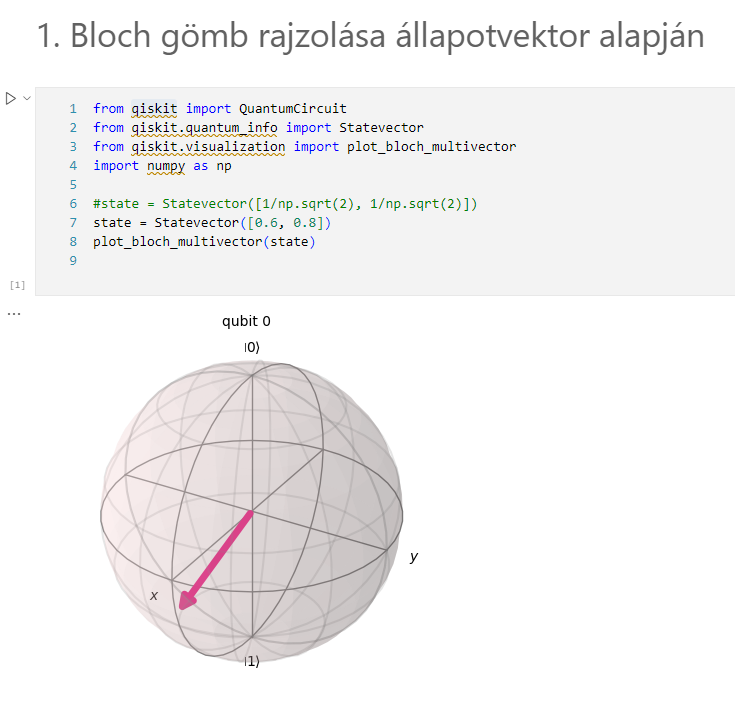
\includegraphics[width=0.9\linewidth]{Simulators/Qiskit.png} 
\end{wrapfigure}

Jupyter környezetben a gyakorlat során ismerkedtünk meg az IBM eszközével. Nem kifejezetten Bloch-gömb szimulátornak tervezték, de sok funkcióval rendelkezik, amik ezt a használati módot is lehetővé teszik.

Előny:

\begin{itemize}
    \item A kapuk helyesen működnek, könnyen paraméterezhetők.
    \item Bármilyen állapotú Qubit-et használhatunk.
    \item Könnyen átlátható.
    \item Szimulációk is futtathatók.
    \item Komplikáltabb feladatokra is használható.
\end{itemize}

Hátrány:

\begin{itemize}
    \item A környezetet telepíteni kell.
    \item Nem valósidőben látjuk a változást.
    \item A kapuk hatása nehezebben követhető.
    \item Több állapot megjelenítésére külön gömböket használ.
\end{itemize}


% Bits and electrons
\vspace{0.4cm}
\subsection{Bits And Electrons}
\textbf{Forrás: \href{https://bits-and-electrons.github.io/bloch-sphere-simulator/}{bits-and-electrons.github.io/bloch-sphere-simulator/}}

Egy webes bloch gömb szimulátor, amely a kapuk bemutatására fókuszál.

Előny:

\begin{itemize}
    \item A kapuk hatását animációval mutatja.
    \item Valós időben láthatjuk az állapotot.
    \item Saját kapuk létrehozása vektor és forgatási szög megadásával.
    \item Előre definiált kapuk: X,Y,Z,H.
    \item Előre definiált fél/negyed/nyolcad fordulat kapuk.
    \item Lambda kapuk: X és Y tengely körül pontos szöggel forgatás.
\end{itemize}

Hátrány:

\begin{itemize}
    \item Csak 1 qubit ábrázolása.
    \item Nem írható be a kiinduló állapot a felhasználói felületen keresztül.
    \item Csak kapuk segítségével lehet módosítani az állapotot.
    \item Hiába animálja a kapukat, az utukat nem rajzolja be, sok kapunál nehezebben lekövethető.
    \item Nehezen állítható alaphelyzetbe. Ki kell törölni a linkből a tulajdonságokat.
    \item Néha eltűnnek bizonyos grafikai elemek.
\end{itemize}

% Bloch kerp
\vspace{0.4cm}
\subsection{Bloch Kerb}
\textbf{Forrás: \href{https://bloch.kherb.io/}{bloch.kherb.io}}

Előny:

\begin{itemize}
    \item Vizualizálja a műveletek útját így könnyebben elképzelhető.
    \item Saját kapuk létrehozása forgatási szögek megadásával.
    \item Forgatási tengely és a régebbi lépések színei is állíthatók.
    \item Állítható, hogy hány hamarabbi lépést mutasson.
    \item Vissza lehet vonni a korábban megtett léptetéseket.
    \item Könnyen alaphelyzetbe állítható.
\end{itemize}

Hátrány:

\begin{itemize}
    \item Csak 1 qubit ábrázolása.
    \item Nem írhatóak be az egyes állapotok UI-n keresztül.
    \item Csak előre definiált kapuk használhatók.
    \item Minden változtatás után visszaállítja az alapértelmezett nézetre.
    \item Nem mutatja valós időben a hozzá tartozó értékeket.
    \item Nem lehet megadni a qubit kiinduló állapotát.
\end{itemize}


% Attila Kun
\vspace{0.4cm}
\subsection{Attila Kun}
\textbf{Forrás: \href{https://attilakun.net/bloch/}{attilakun.net/bloch}}

Előny:

\begin{itemize}
    \item Vizualizálja a műveletek útját így könnyebben elképzelhető.
    \item Könnyen alaphelyzetbe állítható.
    \item Állítható a kiinduló állapot.
    \item Beállítható azonnal a négy alapértelmezett bázis állapot.
    \item A kiinduló állapot állítható a kurzor segítségével vagy pontos adatokat megadni az UI-n keresztül lehet.
    \item Mátrix megadásával lehet saját kaput létrehozni.
    \item Előre definiált kapuk: X,Y,Z,H
\end{itemize}

Hátrány:

\begin{itemize}
    \item Csak 1 qubit ábrázolása.
    \item Az irányítás nem teljesen egyértelmű.
    \item Nem lehet több kaput alkalmazni.
    \item Nem jelenik meg a gömb.
\end{itemize}

% Spec
\newpage
\section{Szoftverkövetelmény specifikáció}

\subsection{Cél}
A szoftver fő célja, hogy könnyen átláthatóan, felhasználó barát módon vizualizálja a Bloch gömböt, ahol könnyen állíthatjuk a kapukat és a qubiteket.

\subsection{Részletes feladatok}
A programban könnyedén lehet qubiteket hozzáadni, módosítani a kiinduló állapotaikat. Öt különböző beépített kapu típus van: X, Y, Z, Hadamard és Phase. A kapuknál van lehetőség létrehozni, sorrenden változtatni, törölni, egybecsatolni és a Phase kapunak paramétereit változtatni. A léptetés útvonala be van rajzolva és lehet állítani a qubit és a hozzátartozó útvonal színét. A qubiteknek lehet különböző színeket adni. Megjeleníti a ket0/1/-/+ bázis állapotokat. 
\newline
itt a hely: majd itt valahol hagyjatok helyet a figma design linkjének meg képnek
...

% Fejlesztői környezet
\newpage
\section{Fejlesztőkörnyezet megnevezése}

\begin{itemize}
    \item \textbf{Godot:}  Godot game engine mellett döntöttünk, mivel könnyen használható, könnyűvé teszi a pluginok használatát és nyílt forráskodú. A saját programozási nyelvében, a \href{https://docs.godotengine.org/en/stable/tutorials/scripting/gdscript/gdscript_basics.html}{gdscript}-ben már sok funkció implementálva van, ami segít nekünk a program elkészítésében. Ebben a környezetben tervezzük leprogramozni a megjelenítéshez szükséges logikát és shadereket.
    \item \textbf{ImGui for Godot:} a godot beépített UI rendszerét nem találtuk alkalmasnak a feladatra, ezért hosszas keresés után az \href{https://godotengine.org/asset-library/asset/2985}{ImGui} mellett döntöttünk. Ezzel a könyvtárral lehetséges megvalósítani a kapuk cserélgetését, a színválasztót, a pop-up ablakok megjelenítését és a saját bemeneti mezők alkalmazását.
    \item \textbf{Egyéb fejlesztéshez használt eszközök:} Visual Studio Code, Git, GitHub, Overleaf
\end{itemize}

\end{document}